\documentclass{article}
\usepackage[utf8]{inputenc}
\usepackage[T1]{fontenc}
\usepackage{graphicx}
\usepackage{hyperref}
\usepackage{geometry}
\geometry{margin=1in}

\title{ENGASTRIMYTHI}
\date{Encyclopaedia Britannica (1771)}

\begin{document}
\maketitle

\section*{Historical source}
\textbf{Entry ID:} \texttt{entry-engastrimythi-523} \\
\textbf{Volume ID:} 144850375 \\
\textbf{Character Count:} 633

\subsection*{Extracted Text}
ENGASTRIMYTHI, in Pagan theology, the Py- thins, or profiledles of Apollo, who delivered oracles from within, without any action of the mouth up lips.

The ancient philophers, \&. are divided upon the fullyelt of the engathyrthd. Hipporcentes mentions is as a idiction. Others will have to kind of strin-tion. Others attribute it to the operation or polefi- tion of an evil finite. And others to antal mecha- nim. M. Scotts maintains that the engathrhythm of the anciens were poets, who, when the prisels could not fpeks, fupplied the defect by explaining in verfe what Apollo dictated in the cavity of the balon on the farced tripod.



\section*{Source record}
\begin{itemize}
\item \textbf{Dataset:} \texttt{NationalLibraryOfScotland/encyclopaedia\_britannica\_illustrated}
\item \textbf{Dataset Revision:} \texttt{309f765b1ecc83e0a7f7762e44b4a927a7555443}
\item \textbf{Page ID:} \texttt{britannica:309f765b1ecc83e0a7f7762e44b4a927a7555443:train:523} \\
  \textbf{Filename:} \texttt{page-0523-a583606e375a.jpg} \\
  \textbf{Row Index:} 523 \\
  \textbf{SHA256:} \texttt{a583606e375ad92d...}
\end{itemize}

\begin{figure}[h]
\centering
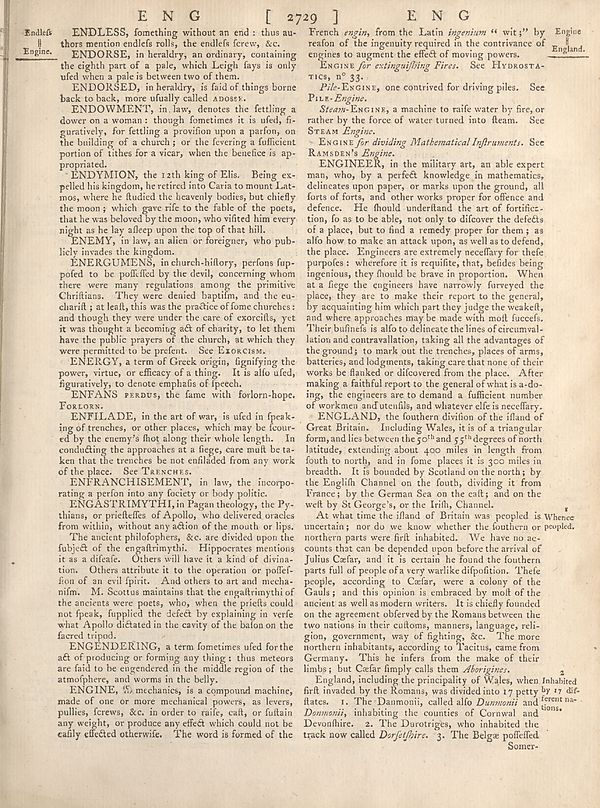
\includegraphics[width=0.85\textwidth]{../scans/page-0523-a583606e375a.jpg}
\caption*{Source scan: \texttt{page-0523-a583606e375a.jpg}}
\end{figure}

\end{document}
